\documentclass[
12pt, % Main document font size
a4paper, % Paper type, use 'letterpaper' for US Letter paper
oneside, % One page layout (no page indentation)
%twoside, % Two page layout (page indentation for binding and different headers)
headinclude,footinclude, % Extra spacing for the header and footer
BCOR5mm, % Binding correction
]{scrartcl}

%%%%%%%%%%%%%%%%%%%%%%%%%%%%%%%%%%%%%%%%%
% Arsclassica Article
% Structure Specification File
%
% This file has been downloaded from:
% http://www.LaTeXTemplates.com
%
% Original author:
% Lorenzo Pantieri (http://www.lorenzopantieri.net) with extensive modifications by:
% Vel (vel@latextemplates.com)
%
% License:
% CC BY-NC-SA 3.0 (http://creativecommons.org/licenses/by-nc-sa/3.0/)
%
%%%%%%%%%%%%%%%%%%%%%%%%%%%%%%%%%%%%%%%%%

%----------------------------------------------------------------------------------------
%	REQUIRED PACKAGES
%----------------------------------------------------------------------------------------

\usepackage[
nochapters, % Turn off chapters since this is an article        
beramono, % Use the Bera Mono font for monospaced text (\texttt)
eulermath,% Use the Euler font for mathematics
pdfspacing, % Makes use of pdftex’ letter spacing capabilities via the microtype package
dottedtoc % Dotted lines leading to the page numbers in the table of contents
]{classicthesis} % The layout is based on the Classic Thesis style



\usepackage[T1]{fontenc} % Use 8-bit encoding that has 256 glyphs

\usepackage[utf8]{inputenc} % Required for including letters with accents

\usepackage{graphicx} % Required for including images
\graphicspath{{Figures/}} % Set the default folder for images

\usepackage{enumitem} % Required for manipulating the whitespace between and within lists

\usepackage{lipsum} % Used for inserting dummy 'Lorem ipsum' text into the template

\usepackage{subfig} % Required for creating figures with multiple parts (subfigures)

\usepackage{amsmath,amssymb,amsthm} % For including math equations, theorems, symbols, etc

\usepackage{varioref} % More descriptive referencing


\usepackage{tabularx}
\usepackage{changepage}
%----------------------------------------------------------------------------------------
%	THEOREM STYLES
%---------------------------------------------------------------------------------------

\theoremstyle{definition} % Define theorem styles here based on the definition style (used for definitions and examples)
\newtheorem{definition}{Definition}

\theoremstyle{plain} % Define theorem styles here based on the plain style (used for theorems, lemmas, propositions)
\newtheorem{theorem}{Theorem}

\theoremstyle{remark} % Define theorem styles here based on the remark style (used for remarks and notes)

%----------------------------------------------------------------------------------------
%	HYPERLINKS
%---------------------------------------------------------------------------------------

\hypersetup{
%draft, % Uncomment to remove all links (useful for printing in black and white)
colorlinks=true, breaklinks=true, bookmarks=true,bookmarksnumbered,
urlcolor=webbrown, linkcolor=RoyalBlue, citecolor=webgreen, % Link colors
pdftitle={}, % PDF title
pdfauthor={\textcopyright}, % PDF Author
pdfsubject={}, % PDF Subject
pdfkeywords={}, % PDF Keywords
pdfcreator={pdfLaTeX}, % PDF Creator
pdfproducer={LaTeX with hyperref and ClassicThesis} % PDF producer
} % Include the structure.tex file which specified the document structure and layout

\hyphenation{Fortran hy-phen-ation} % Specify custom hyphenation points in words with dashes where you would like hyphenation to occur, or alternatively, don't put any dashes in a word to stop hyphenation altogether

%----------------------------------------------------------------------------------------
%	TITLE AND AUTHOR(S)
%----------------------------------------------------------------------------------------

\title{\normalfont\spacedallcaps{RPi based autonomous Car}} % The article title
\author{\spacedlowsmallcaps{Fullstack Embedded (2017)}} 
\date{} % An optional date to appear under the author(s)

%----------------------------------------------------------------------------------------

\begin{document}

%----------------------------------------------------------------------------------------
%	HEADERS
%----------------------------------------------------------------------------------------

\renewcommand{\sectionmark}[1]{\markright{\spacedlowsmallcaps{#1}}} % The header for all pages (oneside) or for even pages (twoside)
%\renewcommand{\subsectionmark}[1]{\markright{\thesubsection~#1}} % Uncomment when using the twoside option - this modifies the header on odd pages
\lehead{\mbox{\llap{\small\thepage\kern1em\color{halfgray} \vline}\color{halfgray}\hspace{0.5em}\rightmark\hfil}} % The header style

\pagestyle{scrheadings} % Enable the headers specified in this block

%----------------------------------------------------------------------------------------
%	TABLE OF CONTENTS & LISTS OF FIGURES AND TABLES
%----------------------------------------------------------------------------------------

\maketitle % Print the title/author/date block

\setcounter{tocdepth}{2} % Set the depth of the table of contents to show sections and subsections only

\tableofcontents % Print the table of contents

\listoffigures % Print the list of figures

\listoftables % Print the list of tables

%----------------------------------------------------------------------------------------
%	ABSTRACT
%----------------------------------------------------------------------------------------

\section*{Abstract} % This section will not appear in the table of contents due to the star (\section*)
The purpose of this document is to give the reader an overview about the RpiCar 's hardware. RpiCar will be used as learning plattform for FSE 2017. The principal hardware's components and interface will be briefly described.

%
\newpage
%

%----------------------------------------------------------------------------------------
%	INTRODUCTION
%----------------------------------------------------------------------------------------

\section{Introduction}
Goal of FSE 2017 will be to build with the students an autonomous car with obstacle avoidanve capability.

%----------------------------------------------------------------------------------------
%	MECHANIC
%----------------------------------------------------------------------------------------

\section{RpiCar 's mechanic}
As shown in Figure~\vref{fig:Mechanic1} and ~\vref{fig:Mechanic2}, mechanical structure is simple and easy to build. The kit can be used with other sensors and actuators to realize obstacle avoidance or wireless remote control. It includes:
\begin{itemize}
\item 1 x Car Chassis 
\item 2 x Gear Motor(1:48) 
\item 2 x Car Tire 
\item 2 x Speed Encoder 
\item 2 x Fastener 
\item 1 x Universal Wheel 
\item 1 x Battery Box 
\item All Necessary Screw And Nut
\end{itemize}

\begin{figure}[!htb]
\minipage{0.48\textwidth}
  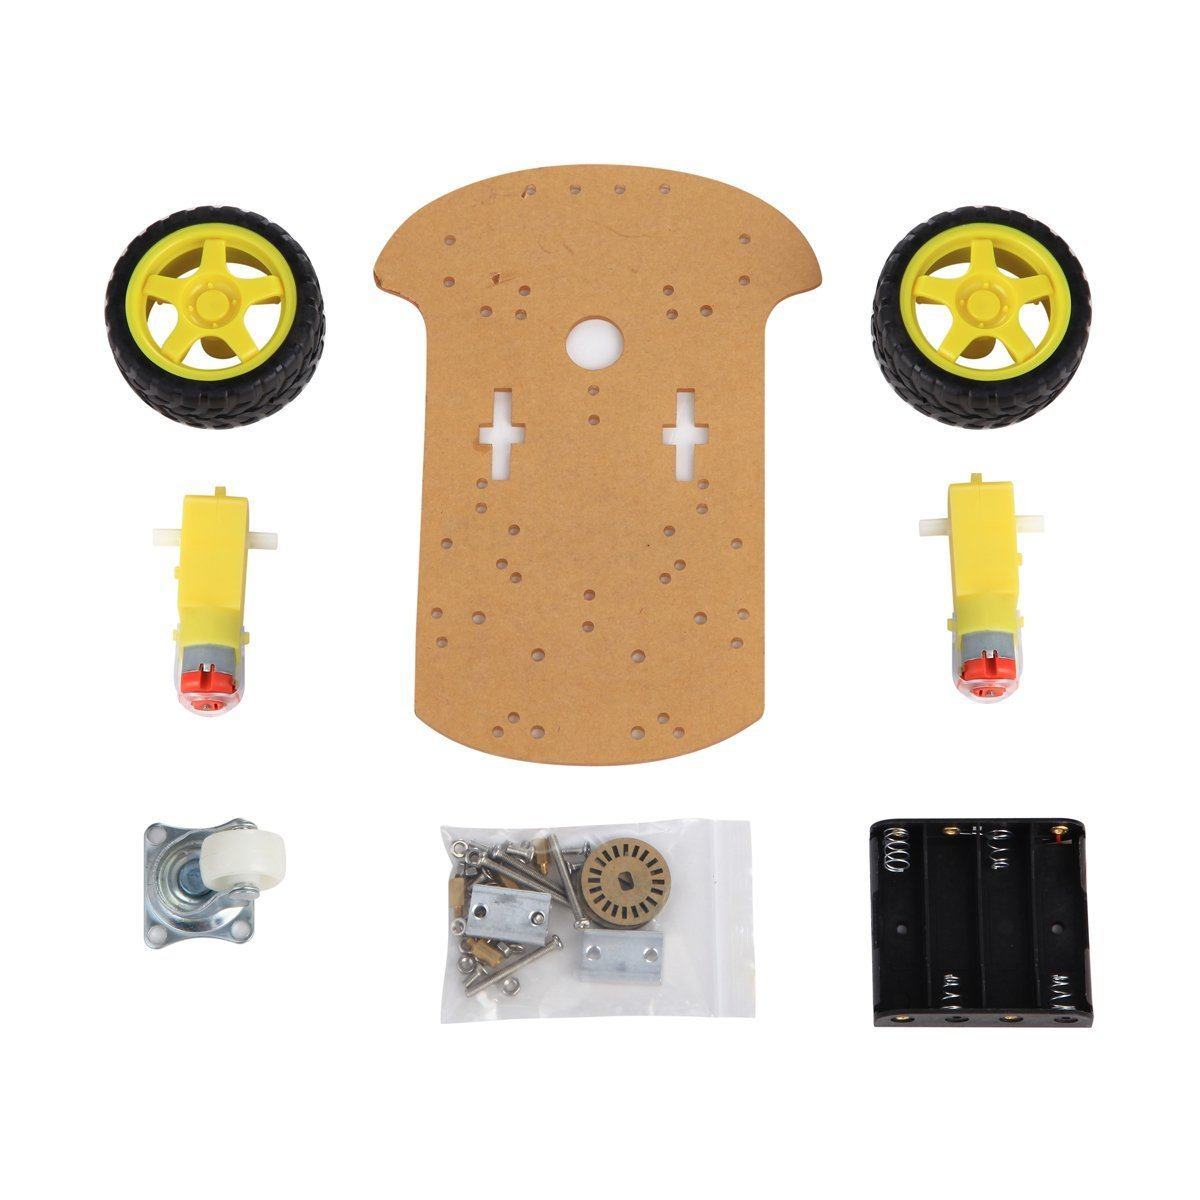
\includegraphics[width=\linewidth]{Mechanic2.png}
  \caption{Robot's components}\label{fig:Mechanic2}
\endminipage\hfill
\minipage{0.48\textwidth}
  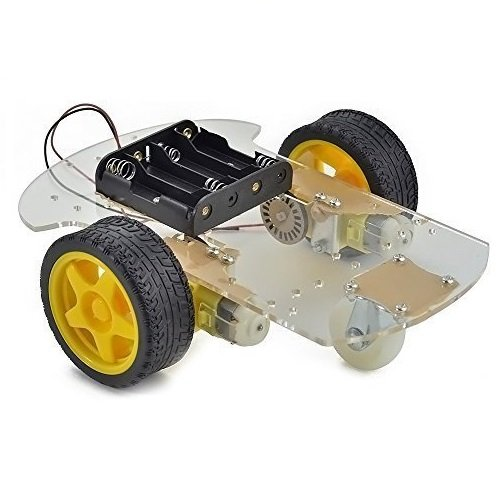
\includegraphics[width=\linewidth]{Mechanic1.png}
  \caption{Assembled robot}\label{fig:Mechanic1}
\endminipage
\end{figure}


%----------------------------------------------------------------------------------------
%	ELECTRONIC
%----------------------------------------------------------------------------------------
\section{RpiCar 's electronic}
\subsection{Analog Inputs for Raspberry Pi Using the MCP3004}
The MCP3008 is a low cost 4-channel 10-bit analog to digital converter.  with 4 channels. The MCP3004 connects to the Raspberry Pi using a SPI serial connection. You can use either the hardware SPI bus (remember to connect GPIO07 and GPIO25 together), or any four GPIO pins and software SPI to communicate to the MCP3004. Software SPI is a little more flexible since it can work with any pins on the Pi, whereas hardware SPI is slightly faster but less flexible because it only works with specific pins. The RpiCar board gives the possibility to try both methods since it is wired to the raspberry pi hardware SPI.

\begin{figure}[!htb]
\centering
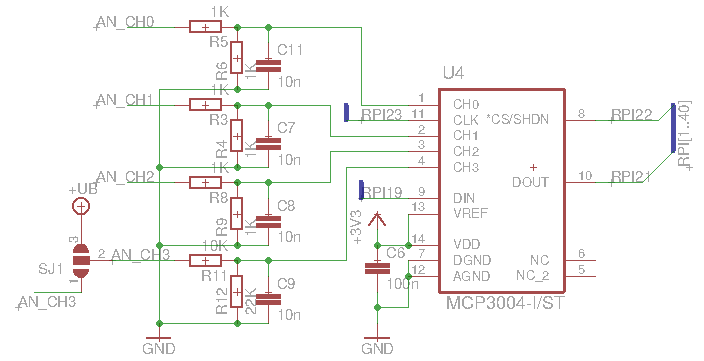
\includegraphics[width=1\columnwidth]{MPC3004} 
\caption[MPC3004 schematic]{MPC3004 schematic}
\label{fig:MPC3004}
\end{figure}

\begin{table}[hbt]
\caption{MCP3004 SPI connection}
\centering
\begin{tabular}{lr}
\toprule
SPI Pins & Raspberry Pi pin \\
\midrule
SCLK (Serial Clock)        & GPIO11 \\
MOSI (Master Out Slave In) & GPIO10 \\
MISO (Master In Slave Out) & GPIO09 \\
CS   (Chip Select)         & GPIO25 \\
\bottomrule
\end{tabular}
\label{tab:label}
\end{table}
Voltage that are allowed to be connected to the MCP3004 have to be selected so that \(V_{out}\) muss be less than 3.3V(\(V_{ref}\)). \(V_{out}\) is the voltage that can be measured after the voltage dividers. All channels except channel 3 are designed to have a measuring range of 0-5V DC. Channel 3 can mesaure up to 10V.
\(V_{out[0-2]}\) for channels 0,1,2 can be calculated as:

\[ V_{ out[0-2] } = \frac{ R_{6} }{ R_{5} + R_{6} } * V_{in}  = 0.5* V_{in}\]

In case of channel 3:

\[ V_{out[3]} = 0.316 * V_{in}\]

Please note that the analog channel 3 is connected per default via a jumper (SJ1) to the robot's supply voltage. Remove the jumper to be able to connect another voltage source to channel 3. 

\subsection{8-channel Bi-directional Logic Level Converter - TXB0108}
Precautions have to be taken when connecting 5V devices to the raspberry pi because it'is vot 5V tolerant. There are many simple ways to handle this issue like voltage dividers.Handling bidirectional signals or high speed transfers can be tough.That's where this lovely chip, the TXB0108 bi-directional level converter comes in! This chip perform bidirectional level shifting from pretty much any voltage to any voltage and will auto-detect the direction 

\begin{figure}[!htb]
\centering
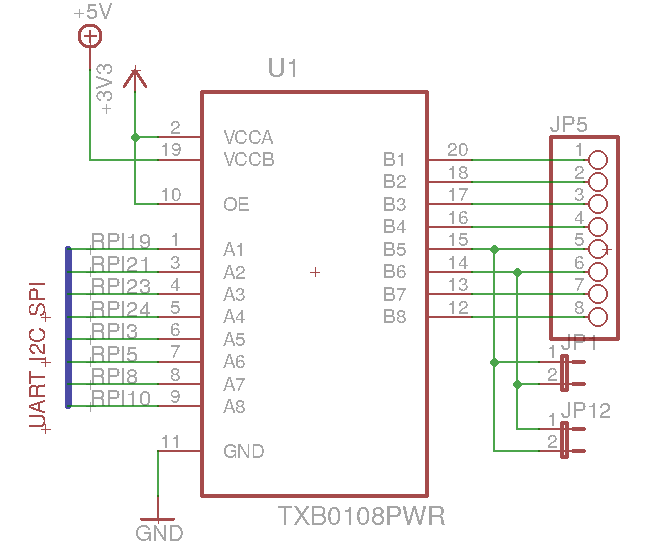
\includegraphics[width=0.8\columnwidth]{TX0108PWR} 
\caption[TX0108PWR schematic]{TX0108PWR schematic}
\label{fig:TX0108PWR}
\end{figure}

\subsection {DC Motor driver - tb6612fng}
The TB6612FNG motor driver can control up to two DC motors at a constant current of 1.2A (3.2A peak). Two input signals (IN1 and IN2) can be used to control the motor in one of four function modes - CW, CCW, short-brake, and stop. The two motor outputs (A and B) can be separately controlled, the speed of each motor is controlled via a PWM input signal with a frequency up to 100kHz. The STBY pin should be pulled high to take the motor out of standby mode.

Logic supply voltage (VCC) can be in the range of 2.7-5.5VDC, while the motor supply (VM) is limited to a maximum voltage of 15VDC. The output current is rated up to 1.2A per channel (or up to 3.2A for a short, single pulse).

Features:
\begin{itemize}
\item[•] Power supply voltage: VM=15V max, VCC=2.7-5.5V
\item[•] Output current: Iout=1.2A(average) / 3.2A (peak)
\item[•] Standby control to save power
\item[•] CW/CCW/short brake/stop motor control modes
\item[•] Built-in thermal shutdown circuit and low voltage detecting circuit
\item[•] All pins of the TB6612FNG broken out to 0.1" spaced pins
\item[•] Filtering capacitors on both supply lines
\end{itemize}

\begin{figure}[!htb]
\centering
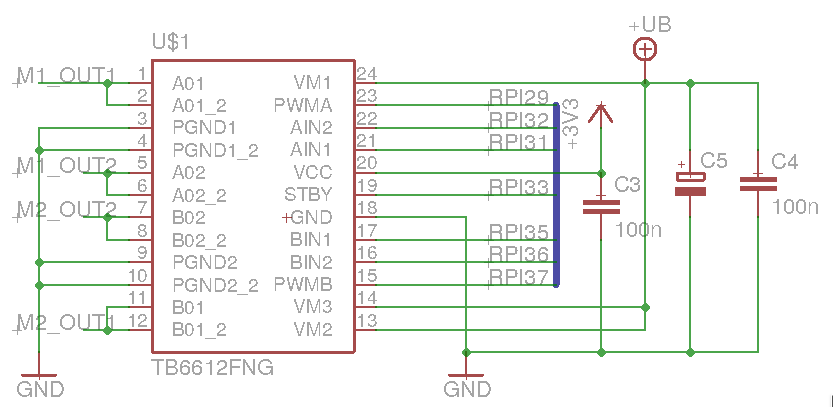
\includegraphics[width=1\columnwidth]{TB6612FNG} 
\caption[TB6612FNG schematic]{TB6612FNG schematic}
\label{fig:TB6612FNG}
\end{figure}
Let’s discuss the pinout for the TB6612FNG:


\newcolumntype{b}{X}
\newcolumntype{s}{>{\hsize=.3\hsize}X}
\newcolumntype{m}{>{\hsize=.5\hsize}X}

\begin{table}[hbt]
\caption{MCP3004 SPI connection}
\centering
\begin{adjustwidth}{-1cm}{}
\resizebox{16cm}{!} {%
\begin{tabularx}{18cm}{smb}
\toprule
Pin Label & Function & Notes \\
\midrule
VM & Motor Voltage  & This is where you provide power for the motors (2.2V to 13.5V)\\
VCC & Logic Voltage & This is the voltage to power the chip and talk to the microcontroller (2.7V to 5.5V)\\
GND & Ground  & Common Ground for both motor voltage and logic voltage (all GND pins are connected)\\
STBY & Standby & Allows the H-bridges to work when high (has a pulldown resistor so it must actively pulled high)\\
AIN1/BIN1 & Input 1 for channels A/B   & One of the two inputs that determines the direction\\
AIN2/BIN2 & Input 2 for channels A/B   & One of the two inputs that determines the direction\\
PWMA/PWMB & PWM input for channels A/B & PWM input that controls the speed\\
A01/B01 & Output 1 for channels A/B  & One of the two outputs to connect the motor\\
A02/B02 & Output 2 for channels A/B  & One of the two outputs to connect the motor\\
\bottomrule
\end{tabularx} } 
\end{adjustwidth}
\label{tab:label}
\end{table}

When the outputs are set to High/Low your motor will run. When they are set to Low/High the motor will run in the opposite direction. In both cases, the speed is controlled by the PWM input.

\begin{table}[hbt]
\caption{MCP3004 SPI connection}
\centering
\begin{tabular}{llllll}
\toprule
In1  & In2 & PWM & Out1 & Out2 & Mode \\
\midrule
H    & H   & H/L & L    &L     & Short brake\\
L    & H   & H   & L    & H    & CCW\\
L    & H   & L   & L    & L    & Short brake\\
H    & L   & H   & H    & L    & CW\\
H    & L   & L   & L    & L    & Short brake\\
L    & L   & H   & OFF  & OFF  & Stop\\
\bottomrule
\end{tabular}
\label{tab:label}
\end{table}














\end{document}

